\PassOptionsToPackage{unicode=true}{hyperref} % options for packages loaded elsewhere
\PassOptionsToPackage{hyphens}{url}
\documentclass[11pt,ignorenonframetext,aspectratio=169]{beamer}
\IfFileExists{pgfpages.sty}{\usepackage{pgfpages}}{}
\setbeamertemplate{caption}[numbered]
\setbeamertemplate{caption label separator}{: }
\setbeamercolor{caption name}{fg=normal text.fg}
\beamertemplatenavigationsymbolsempty
\usepackage{lmodern}
\usepackage{amssymb,amsmath}
\usepackage{ifxetex,ifluatex}
\usepackage{fixltx2e} % provides \textsubscript
\ifnum 0\ifxetex 1\fi\ifluatex 1\fi=0 % if pdftex
  \usepackage[T1]{fontenc}
  \usepackage[utf8]{inputenc}
\else % if luatex or xelatex
  \ifxetex
    \usepackage{mathspec}
  \else
    \usepackage{fontspec}
\fi
\defaultfontfeatures{Ligatures=TeX,Scale=MatchLowercase}







\fi

  \usetheme[sectionpage=progressbar, titleformat=regular,
numbering=counter, block=fill]{metropolis}






% use upquote if available, for straight quotes in verbatim environments
\IfFileExists{upquote.sty}{\usepackage{upquote}}{}
% use microtype if available
\IfFileExists{microtype.sty}{%
  \usepackage{microtype}
  \UseMicrotypeSet[protrusion]{basicmath} % disable protrusion for tt fonts
}{}


\newif\ifbibliography


\hypersetup{
      pdftitle={Domestication, plant introduction, and acclimatization},
        pdfauthor={Deependra Dhakal},
          pdfborder={0 0 0},
    breaklinks=true}
%\urlstyle{same}  % Use monospace font for urls







% Prevent slide breaks in the middle of a paragraph:
\widowpenalties 1 10000
\raggedbottom

  \AtBeginPart{
    \let\insertpartnumber\relax
    \let\partname\relax
    \frame{\partpage}
  }
  \AtBeginSection{
    \ifbibliography
    \else
      \let\insertsectionnumber\relax
      \let\sectionname\relax
      \frame{\sectionpage}
    \fi
  }
  \AtBeginSubsection{
    \let\insertsubsectionnumber\relax
    \let\subsectionname\relax
    \frame{\subsectionpage}
  }



\setlength{\parindent}{0pt}
\setlength{\parskip}{6pt plus 2pt minus 1pt}
\setlength{\emergencystretch}{3em}  % prevent overfull lines
\providecommand{\tightlist}{%
  \setlength{\itemsep}{0pt}\setlength{\parskip}{0pt}}

  \setcounter{secnumdepth}{0}


  \usepackage{setspace}
  \usepackage{wasysym}
  % \usepackage{fontenc}
  \usepackage{booktabs,siunitx}
  \usepackage{longtable}
  \usepackage{array}
  \usepackage{multirow}
  \usepackage{wrapfig}
  \usepackage{float}
  \usepackage{colortbl}
  \usepackage{pdflscape}
  \usepackage{tabu}
  \usepackage{threeparttable}
  \usepackage{threeparttablex}
  \usepackage[normalem]{ulem}
  \usepackage{makecell}
  \usepackage{xcolor}
  \usepackage{tikz} % required for image opacity change
  \usepackage[absolute,overlay]{textpos} % for text formatting
  \usepackage[skip=0.333\baselineskip]{caption}
  % \usepackage{newtxtext,newtxmath}% better than txfonts   
  \usepackage[english]{babel}
  \usepackage{pgfpages}

  \sisetup{per-mode=symbol}

  % % Added by CII
  % \usepackage[format=hang,labelfont=bf,margin=0.5cm,justification=centering]{caption}
  % \captionsetup{font=small,width=0.9\linewidth,labelfont=small,textfont={small}}
  % % End of CII addition

  % \usepackage{subcaption}
  % \newcommand{\subfloat}[2][need a sub-caption]{\subcaptionbox{#1}{#2}}

  \captionsetup[sub]{font=footnotesize,labelfont=footnotesize,textfont=footnotesize}
  % \captionsetup[subfigure]{font=small,labelfont=small,textfont=small}
  % \captionsetup[subfloat]{font=scriptsize,labelfont=scriptsize,textfont=scriptsize}

  % this font option is amenable for beamer, although these are global settings
  \setbeamerfont{caption}{size=\tiny}
  % \setbeamerfont{subcaption}{size=\tiny} % this does not chage subfloat fonts
  % \setbeamerfont{subfloat}{size=\tiny} % this does not change subfloat fonts
   
   % use single line spacing ?
  \singlespacing

  % use cslreferences environment
  % this is revised as of Oct, 2022 (https://stackoverflow.com/questions/59193797/pandocs-environment-cslreferences-undefined-when-knitting-rmarkdown-to-pdf-in-r)
  \newlength{\cslhangindent}
  \setlength{\cslhangindent}{1.5em}
  \newenvironment{CSLReferences}%
    {\setlength{\parindent}{0pt}%
    \everypar{\setlength{\hangindent}{\cslhangindent}}\ignorespaces}%
    {\par}

  \title[]{Domestication, plant introduction, and acclimatization}


  \author[
        Deependra Dhakal
    ]{Deependra Dhakal}

  \institute[
    ]{
    Agriculture and Forestry University\\
\textit{ddhakal.rookie@gmail.com}\\
\url{https://rookie.rbind.io}
    }

\date[
      
  ]{
    }


\begin{document}

% Hide progress bar and footline on titlepage
  \begin{frame}[plain]
  \titlepage
  \end{frame}



\hypertarget{domestication}{%
\section{Domestication}\label{domestication}}

\begin{frame}{What is a weed?}
\protect\hypertarget{what-is-a-weed}{}
\begin{itemize}
\tightlist
\item
  ``A plant in the wrong place''
\item
  How accurate is the definition ?
\item
  We define weeds as plants we do not want that compete for resources
  with those we do want.
\item
  Clearly we have criteria about which plants we want and those that
  fail those criteria.
\item
  In evolutionary terms, it is the cultivated plants that are ``fitter''
  than the weeds, as they have characteristics which we want, and since
  in the fi eld and the garden we have largely substituted ourselves for
  nature, and here it is us who control the evolutionary process.
\item
  However, many commercially grown plants survive as volunteer weeds, or
  ``escapes,'' in either the same, or different, regions to those in
  which they are most commonly grown commercially.
\end{itemize}
\end{frame}

\begin{frame}{Domestication}
\protect\hypertarget{domestication-1}{}
\begin{columns}[T,onlytextwidth]
\column{.6\linewidth}

  \begin{block}{Domestication}

"The gap between the wild and the cultivated is all about the difference between nature's requirements and ours." -- @kingsbury2009hybrid

"A plant population has been domesticated when it has been substantially altered from the wild state and certainly when it has been so altered to be unable to survive in the wild" -- N.W. Simmonds
  \end{block}

Domestication is the process by which genetic changes (shifts) in wild plants are brought about through a selection process imposed by humans.

\column{0.4\textwidth}

\begin{figure}

{\centering 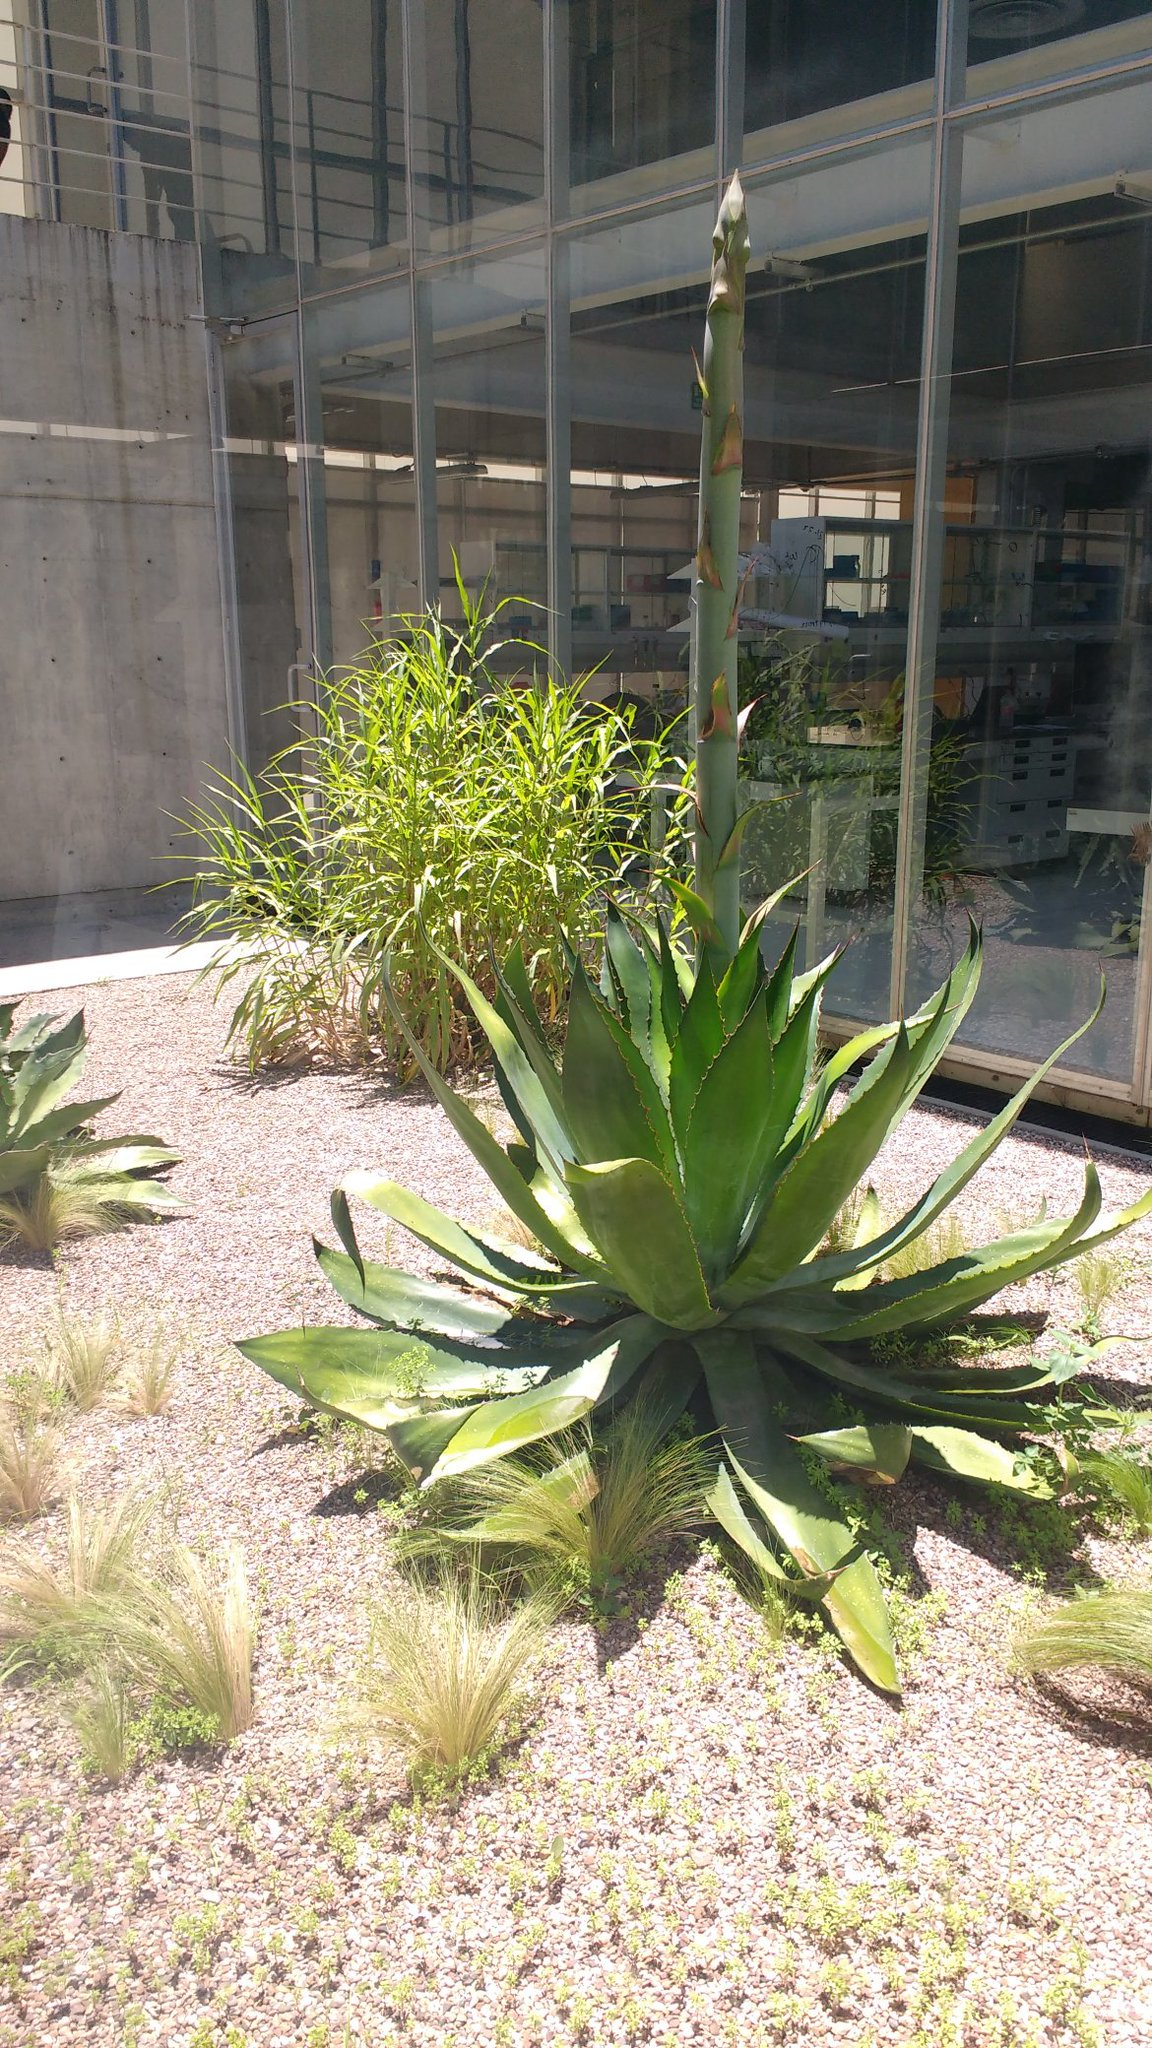
\includegraphics[width=0.7\textwidth, keepaspectratio,height=0.92\textheight]{./images/Perennial_teosinte} 

}

\caption{Perennial teosinte}\label{fig:weed-vs-crop}
\end{figure}

\end{columns}
\end{frame}

\begin{frame}{}
\protect\hypertarget{section}{}
\begin{itemize}
\tightlist
\item
  Because of the roles of humans (\emph{Domesticators}), the process
  results characteristics that are beneficial to humans but some that
  would be disadvantageous for plants in their natural habitats.
\item
  Results are the plants that are adapted to supervised cultural
  conditions and which posses characteristics that are preferred by
  producers and consumers.
\item
  E.g. Modern corn stripped is completely of its seed dispersal ability.
\item
  Both wild and domesticated populations are subject to evolution
\item
  Forces of selection determine what will be domesticated and that which
  will continue in wild

  \begin{itemize}
  \tightlist
  \item
    The natural selection favours plant phenotypes which have the
    greatest chance of survival, reproduction, and distribution of
    progeny.
  \item
    Human selection is the result of conscious decisions by a farmer or
    plant breeder to keep the progeny of a particular parent and discard
    others.
  \end{itemize}
\end{itemize}
\end{frame}

\begin{frame}{Evolution}
\protect\hypertarget{evolution}{}
\begin{itemize}
\tightlist
\item
  The process by which new species are formed from preexisting species
  over a period of time.
\item
  Previously, plant breeding and evolution were considered similar
  processes, considering that both involve creation of variation and
  selection among the variability.

  \begin{itemize}
  \tightlist
  \item
    Either by human or naturally
  \item
    Mechanisms of change are similar for both (Mutation, selection,
    hybridization and polyploidization)
  \end{itemize}
\item
  Key difference is on the duration of process.
\end{itemize}
\end{frame}

\begin{frame}{Domestication syndrome (Changes in plant species under
domestication)}
\protect\hypertarget{domestication-syndrome-changes-in-plant-species-under-domestication}{}
\begin{table}
\centering\begingroup\fontsize{6}{8}\selectfont

\begin{tabular}{>{\raggedright\arraybackslash}p{18em}>{\raggedright\arraybackslash}p{42em}}
\toprule
General effect & Specific traits altered\\
\midrule
\cellcolor{gray!6}{Increased seedling vigor (more plants germinating)} & \cellcolor{gray!6}{Loss of seed or tuber dormancy}\\
 & Large seeds\\
\cellcolor{gray!6}{Modified reproductive system} & \cellcolor{gray!6}{Increased selfing}\\
 & Reduced complexity of reproductive organs\\
\cellcolor{gray!6}{} & \cellcolor{gray!6}{Vegetatively reproducing plants}\\
\addlinespace
 & Altered photoperiod sensitivity\\
\cellcolor{gray!6}{} & \cellcolor{gray!6}{Shift in sex form of species}\\
 & Promotion of asexual reproduction\\
\cellcolor{gray!6}{Increased number of seeds harvested} & \cellcolor{gray!6}{Non-shattering}\\
 & Reduced number of branches (more fruits per branch)\\
\addlinespace
\cellcolor{gray!6}{Increased appeal to consumers} & \cellcolor{gray!6}{Attractive fruit/seed colors and patterns}\\
 & Enhanced flavor, texture, and taste of seeds/fruits/tubers (food parts)\\
\cellcolor{gray!6}{} & \cellcolor{gray!6}{Reduced toxic principles (safer food)}\\
 & Larger fruits\\
\cellcolor{gray!6}{} & \cellcolor{gray!6}{Reduces spikiness}\\
\addlinespace
 & Increase in economic yield (HI)\\
\cellcolor{gray!6}{Altered plant architecture and growth habit} & \cellcolor{gray!6}{Compact growth habit (Determinacy, reduced plant size, dwarfism)}\\
 & Reduced branching\\
\cellcolor{gray!6}{} & \cellcolor{gray!6}{Decreases in variability within a variety}\\
Change in developmental phenology & Change in life cycle (normally from perennial to annual for seed crops, and from annual to biennial for vegetable crops)\\
\bottomrule
\end{tabular}
\endgroup{}
\end{table}
\end{frame}

\begin{frame}{Wild versus domestication}
\protect\hypertarget{wild-versus-domestication}{}
\begin{columns}[T,onlytextwidth]
\column{0.4\textwidth}

\begin{figure}

{\centering 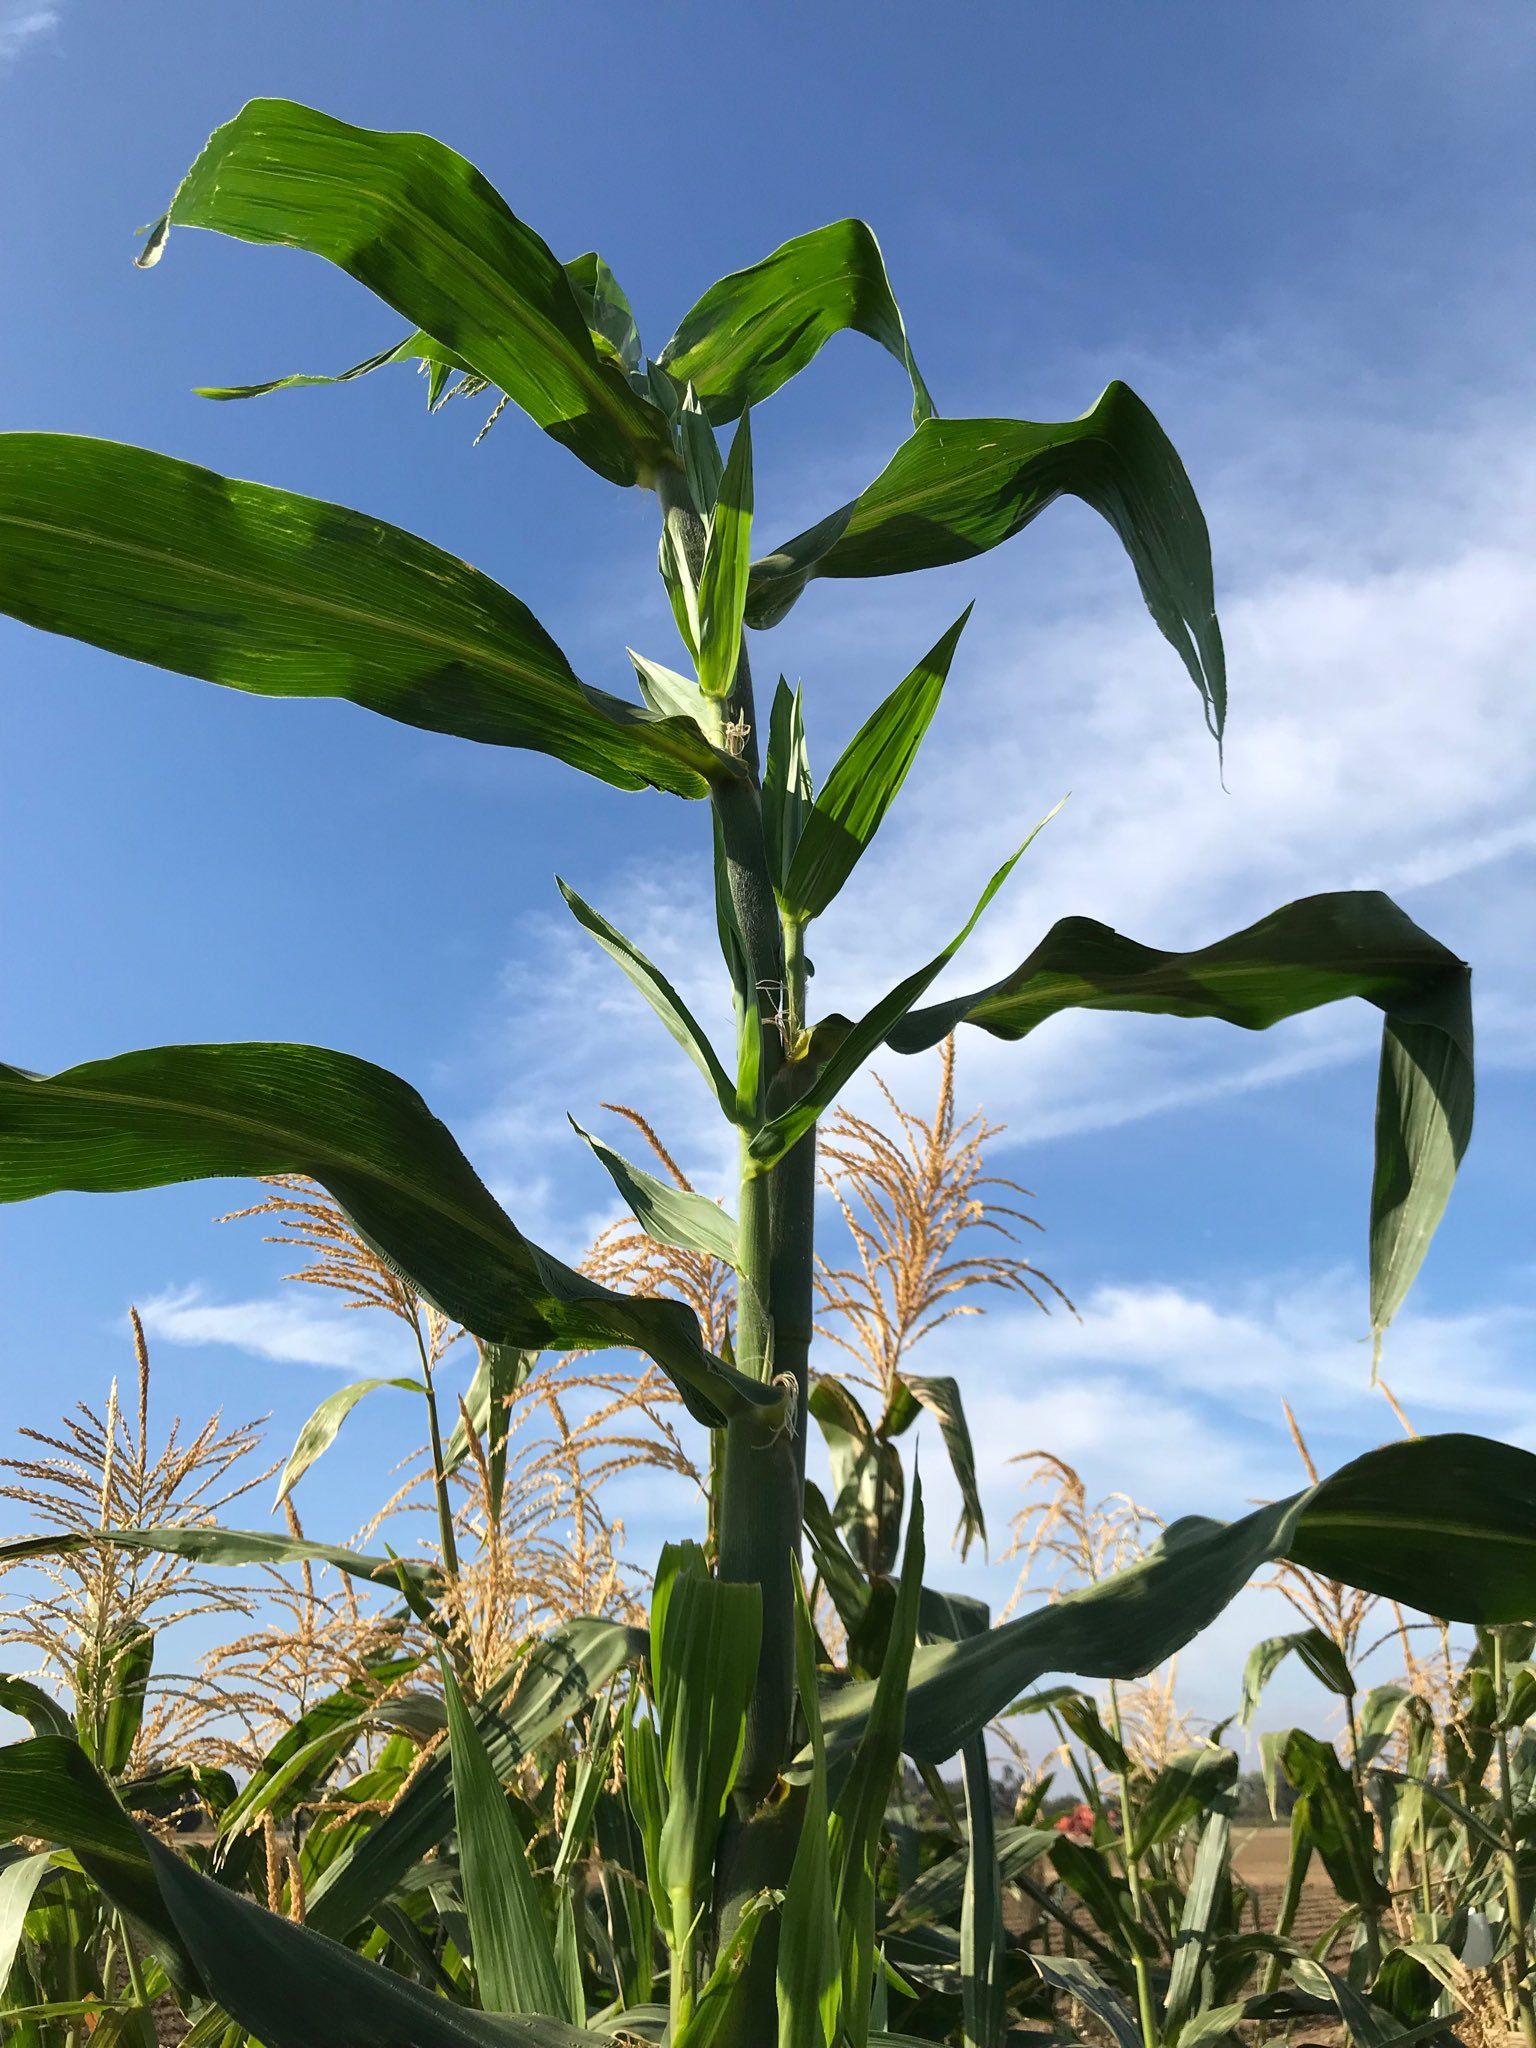
\includegraphics[width=0.7\textwidth, keepaspectratio,height=0.8\textheight]{./images/Teosinte_maize_hybrid_cross} 

}

\caption{Teosinte maize hybrid}\label{fig:unnamed-chunk-1}
\end{figure}

\column{0.6\textwidth}

\begin{figure}
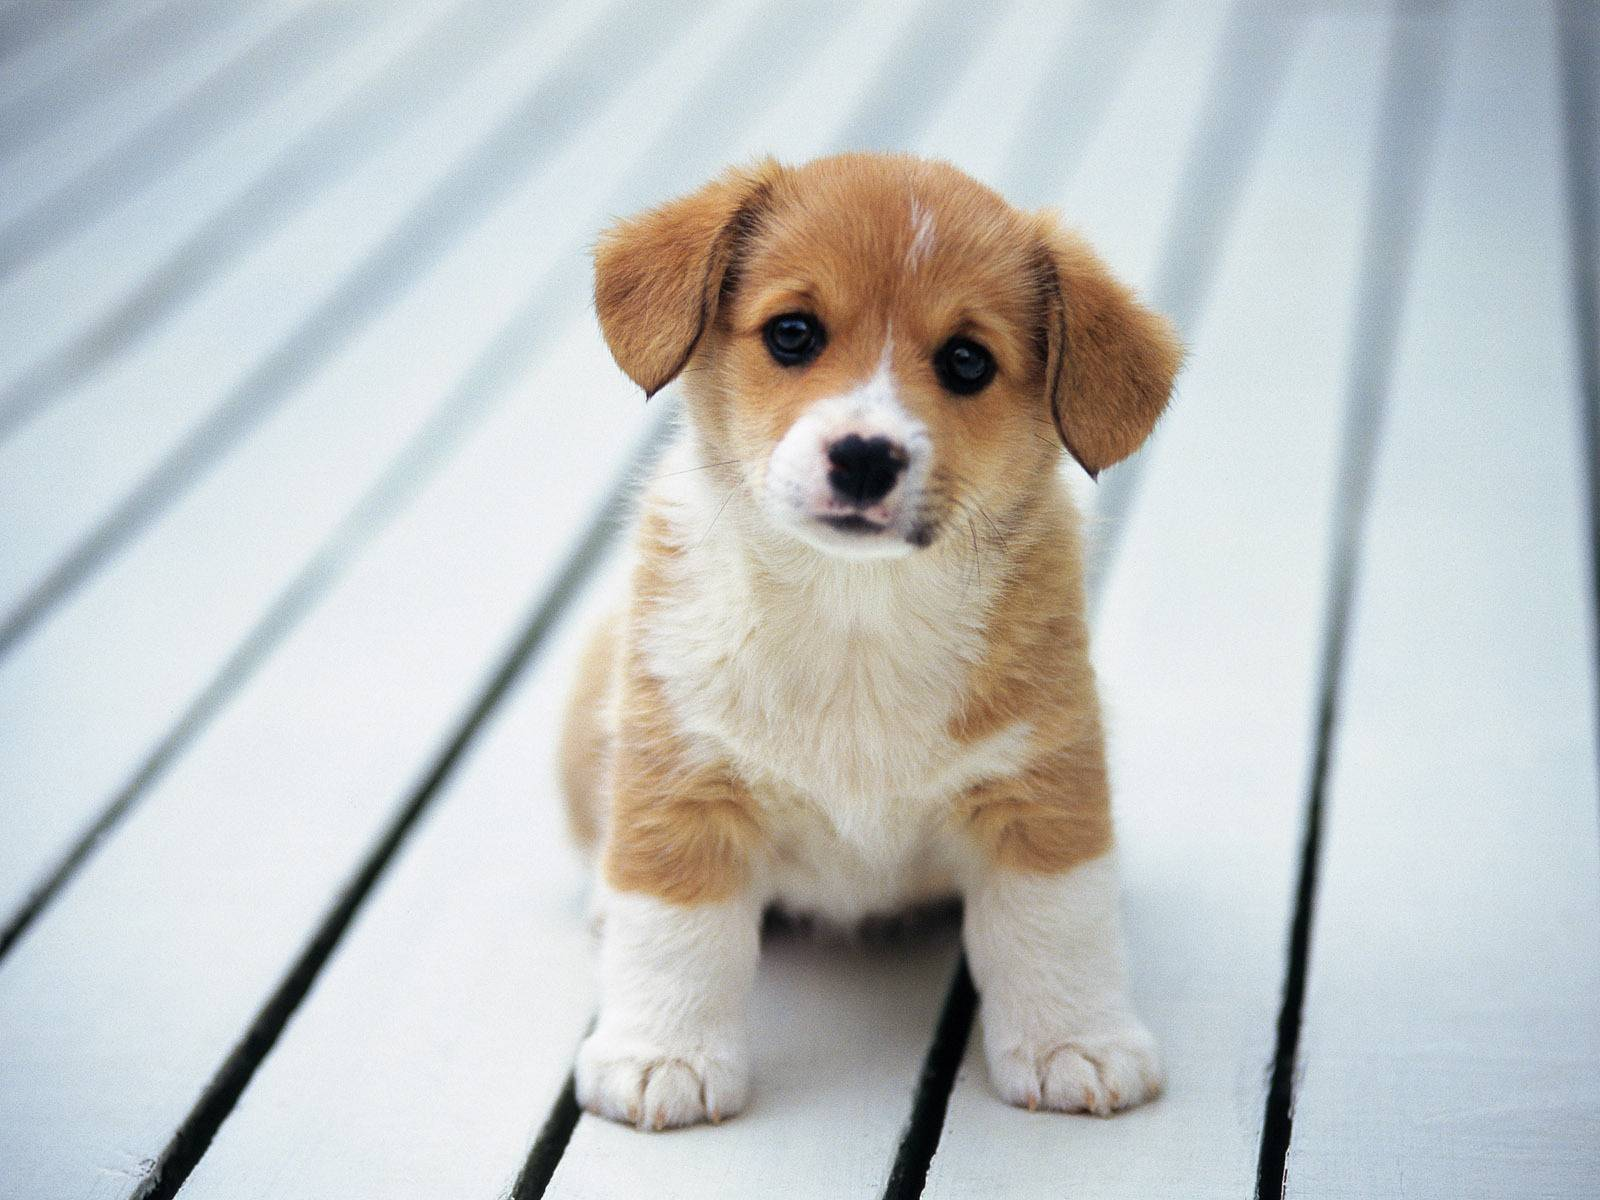
\includegraphics[width=0.4\textwidth, keepaspectratio]{./images/domestic_dog_puppy} \caption{Domesticated dog}\label{fig:domesticated}
\end{figure}


\begin{figure}
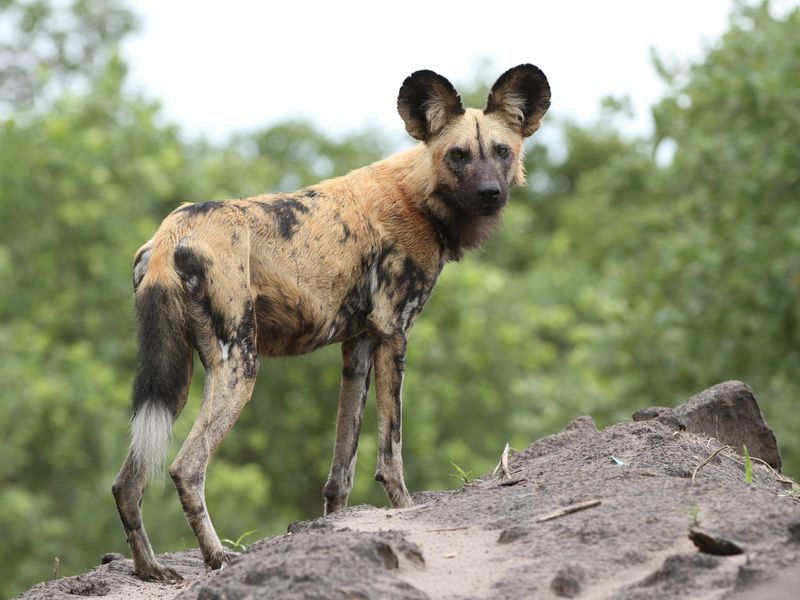
\includegraphics[width=0.4\textwidth, keepaspectratio]{./images/wild_dog_african} \caption{Wild dog}\label{fig:wild}
\end{figure}

\end{columns}
\end{frame}

\begin{frame}{}
\protect\hypertarget{section-1}{}
\begin{figure}
\includegraphics[width=0.7\textwidth, keepaspectratio,height=0.8\textheight]{./images/tomato_wild_domestic} \caption{Wild versus domesticated tomatoes}\label{fig:wild-vs-domesticated-tomato}
\end{figure}
\end{frame}

\begin{frame}{}
\protect\hypertarget{section-2}{}
\begin{itemize}
\item
  Wild cereal plants tend to have many small seeds at maturity and
  disperse their seed by shattering. These seeds also are likely to be
  attached to a strong awn to aid dispersal.
\item
  Similarly, wild potato species produce many small tubers, have their
  tubers develop at the end of very long stolons (so that daughter
  plants do not have to occupy ground too close to the parent), and many
  have tubers with high levels of toxin, which discourage animals from
  eating them.
\item
  Breeders have developed cereal cultivars which have fewer, but larger
  seeds, that do not shatter their seeds at maturity and that have a
  non-persistent awn.
\end{itemize}
\end{frame}

\begin{frame}{}
\protect\hypertarget{section-3}{}
\begin{itemize}
\item
  Similarly potato breeders have selected plants with fewer, but larger
  tubers, shorter stolons and with reduced levels of toxins in the
  tuber.
\item
  Human selection also has produced crops that are more uniform in the
  expression of many of their characteristics. For example, they have
  selected seeds that all mature at the same time, with uniform
  germination, and fruits with uniform fruit size and shape.
\item
  In more recent times plant breeders' selection has tended to result in
  shorter plants, greater harvest index, and increased ease of harvest
  (especially mechanized).
\end{itemize}
\end{frame}

\begin{frame}{Germplasm}
\protect\hypertarget{germplasm}{}
\begin{itemize}
\tightlist
\item
  Germplasm refers to the genetic material that can be used to
  perpetuate a species or population.
\item
  Genetic resources such as seeds or tissues that are maintained for the
  purpose of animal and plant breeding, preservation, and other research
  uses.
\item
  Provides the material used to initiate a breeding program
\item
  Sometimes only germplasm screening and evaluation is practiced for
  introduction of improved variety in a region
\item
  Certain institutional sets-ups such as gene banks are charged with the
  responsibility of assembling, cataloguing, storing and managing large
  number of germplasm. This allows for quick retrieval.
\end{itemize}
\end{frame}

\begin{frame}{Gene pool}
\protect\hypertarget{gene-pool}{}
J.R. Harlan and J.M.J. de Wet proposed a categorization of gene pools of
cultivated crops according to the feasibility of gene transfer or gene
flow from those species to the crop species.

\begin{figure}
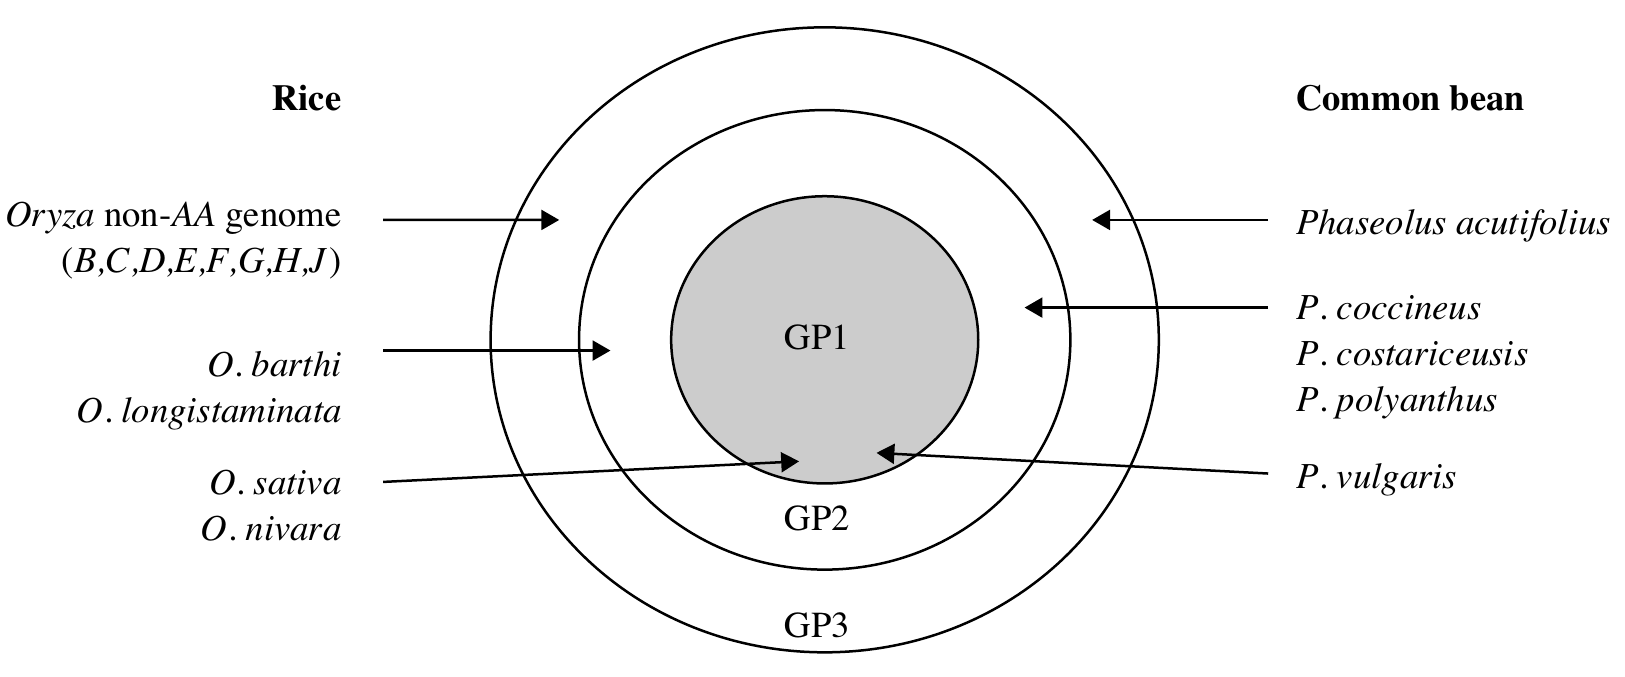
\includegraphics[width=0.7\textwidth, keepaspectratio,height=0.6\textheight]{./images/crop_gene_pools} \caption{Crop gene pools; A system proposed by Harlan}\label{fig:gene-pools}
\end{figure}
\end{frame}

\begin{frame}{Types of gene pool}
\protect\hypertarget{types-of-gene-pool}{}
\begin{itemize}
\tightlist
\item
  \emph{Primary gene pool (GP1)}

  \begin{itemize}
  \tightlist
  \item
    GP1 consists of biological species that can be intercrossed easily
    (interfertile) without any problems with fertility of the progeny.
    That is, there is no restriction to gene exchange between members of
    the group. This group may contain both cultivated and wild
    progenitors of the species.
  \end{itemize}
\item
  \emph{Secondary gene pool (GP2)}

  \begin{itemize}
  \tightlist
  \item
    Members of this gene pool include both cultivated and wild relatives
    of the crop species. They are more distantly related and have
    crossability problems. Nonetheless, crossing produces hybrids and
    derivatives that are sufficiently fertile to allow gene flow. GP2
    species can cross with those in GP1, with some fertility of the F1,
    but more difficulty with success.
  \end{itemize}
\end{itemize}
\end{frame}

\begin{frame}{}
\protect\hypertarget{section-4}{}
\begin{itemize}
\tightlist
\item
  \emph{Tertiary gene pool (GP3)}

  \begin{itemize}
  \tightlist
  \item
    GP3 involves the outer limits of potential genetic resources. Gene
    transfer by hybridization between GP1 and GP3 is very problematic,
    resulting in lethality, sterility, and other abnormalities. To
    exploit germplasm from distant relatives, tools such as embryo
    rescue and bridge crossing may be used to nurture an embryo from a
    wide cross to a full plant and to obtain fertile plants.
  \end{itemize}
\end{itemize}
\end{frame}

\hypertarget{domestication-and-origin-of-major-crop-species}{%
\section{Domestication and origin of major crop
species}\label{domestication-and-origin-of-major-crop-species}}

\begin{frame}{Center of Origin}
\protect\hypertarget{center-of-origin}{}
\begin{table}

\caption{\label{tab:origin-of-crops}Estimated time of domestication and centre of origin of major crop species; @brown2014plant, Page 23}
\centering
\fontsize{6}{8}\selectfont
\begin{tabular}[t]{l>{\raggedright\arraybackslash}p{14em}>{\raggedright\arraybackslash}p{8em}>{\raggedright\arraybackslash}p{22em}}
\toprule
Crop category & Crop & Length of time domesticated (years) & Possible region of origin\\
\midrule
\cellcolor{gray!6}{} & \cellcolor{gray!6}{Maize, Zea mays} & \cellcolor{gray!6}{7000} & \cellcolor{gray!6}{Mexico, Central America}\\
\cmidrule{2-4}
 & Rice, Oryza sativa & 4500 & Thailand, Southern China\\
\cmidrule{2-4}
\cellcolor{gray!6}{} & \cellcolor{gray!6}{Wheat, Triticum spp.} & \cellcolor{gray!6}{8500} & \cellcolor{gray!6}{Syria, Jordan, Israel, Iraq}\\
\cmidrule{2-4}
 & Barley, Hordeum vulgare & 9000 & Syria, Jordan, Israel, Iraq\\
\cmidrule{2-4}
\cellcolor{gray!6}{\multirow{-5}{*}{\raggedright\arraybackslash Cereals}} & \cellcolor{gray!6}{Sorghum, Sorghum bicolor} & \cellcolor{gray!6}{8000} & \cellcolor{gray!6}{Equatorial Africa}\\
\cmidrule{1-4}
 & Soybean, Glycine max & 2000 & North China\\
\cmidrule{2-4}
\cellcolor{gray!6}{} & \cellcolor{gray!6}{Oil palm, Elaeis guineensis} & \cellcolor{gray!6}{9000} & \cellcolor{gray!6}{Central Africa}\\
\cmidrule{2-4}
 & Coconut palm, Cocos nucifera & 100 & Southern Asia\\
\cmidrule{2-4}
\cellcolor{gray!6}{} & \cellcolor{gray!6}{Rapeseed, Brassica napus} & \cellcolor{gray!6}{500} & \cellcolor{gray!6}{Mediterranean Europe}\\
\cmidrule{2-4}
\multirow{-5}{*}{\raggedright\arraybackslash Oilseeds} & Sunflower, Helianthus annus & 3000 & Western United States\\
\bottomrule
\end{tabular}
\end{table}
\end{frame}

\begin{frame}{}
\protect\hypertarget{section-5}{}
\begin{table}

\caption{\label{tab:origin-of-crops2}Estimated time of domestication ...}
\centering
\fontsize{6}{8}\selectfont
\begin{tabular}[t]{l>{\raggedright\arraybackslash}p{14em}>{\raggedright\arraybackslash}p{8em}>{\raggedright\arraybackslash}p{22em}}
\toprule
Crop category & Crop & Length of time domesticated (years) & Possible region of origin\\
\midrule
\cellcolor{gray!6}{} & \cellcolor{gray!6}{Beans, Phaseolus spp} & \cellcolor{gray!6}{7000} & \cellcolor{gray!6}{Centra America, Mexico}\\
\cmidrule{2-4}
 & Lentil, Lens culinaris & 7000 & Syria, Jordan, Israel, Iraq\\
\cmidrule{2-4}
\cellcolor{gray!6}{\multirow{-3}{*}{\raggedright\arraybackslash Pulses}} & \cellcolor{gray!6}{Peas, Pisum sativum} & \cellcolor{gray!6}{9000} & \cellcolor{gray!6}{Syria, Jordan, Israel, Iraq}\\
\cmidrule{1-4}
 & Potato, Solanum tuberosum & 7000 & Peru\\
\cmidrule{2-4}
\cellcolor{gray!6}{} & \cellcolor{gray!6}{Cassava, Manihot esculenta} & \cellcolor{gray!6}{5000} & \cellcolor{gray!6}{Brazil, Mexico}\\
\cmidrule{2-4}
 & Sweet potato, Ipomoea batatas & 6000 & South Central America\\
\cmidrule{2-4}
\cellcolor{gray!6}{\multirow{-4}{*}{\raggedright\arraybackslash Root crops}} & \cellcolor{gray!6}{Sugar beet, Beta vulgaris} & \cellcolor{gray!6}{300} & \cellcolor{gray!6}{Mediterranean Europe}\\
\cmidrule{1-4}
 & Tomato, Lycopersicum esculentum & 3000 & Western South America\\
\cmidrule{2-4}
\cellcolor{gray!6}{} & \cellcolor{gray!6}{Cabbage, Brassica oleracea} & \cellcolor{gray!6}{3000} & \cellcolor{gray!6}{Mediterranean Europe}\\
\cmidrule{2-4}
\multirow{-3}{*}{\raggedright\arraybackslash Vegetables} & Onion, Allium spp. & 4500 & Iran, Afganistan, Pakistan\\
\bottomrule
\end{tabular}
\end{table}
\end{frame}

\begin{frame}{}
\protect\hypertarget{section-6}{}
\begin{table}

\caption{\label{tab:origin-of-crops3}Estimated time of domestication ...}
\centering
\fontsize{6}{8}\selectfont
\begin{tabular}[t]{l>{\raggedright\arraybackslash}p{14em}>{\raggedright\arraybackslash}p{8em}>{\raggedright\arraybackslash}p{22em}}
\toprule
Crop category & Crop & Length of time domesticated (years) & Possible region of origin\\
\midrule
\cellcolor{gray!6}{} & \cellcolor{gray!6}{Orange, Citrus sinensis} & \cellcolor{gray!6}{9000} & \cellcolor{gray!6}{South-east Asia}\\
\cmidrule{2-4}
 & Apple, Malus spp. & 3000 & Asia Minor, Central Asia\\
\cmidrule{2-4}
\cellcolor{gray!6}{} & \cellcolor{gray!6}{Grape, Vitis spp.} & \cellcolor{gray!6}{7000} & \cellcolor{gray!6}{Eastern Asia}\\
\cmidrule{2-4}
\multirow{-4}{*}{\raggedright\arraybackslash Fruit} & Banana, Musa acuminata, M. balbisiana & 4500 & South-east Asia\\
\cmidrule{1-4}
\cellcolor{gray!6}{} & \cellcolor{gray!6}{Cotton, Gossypium spp.} & \cellcolor{gray!6}{4500} & \cellcolor{gray!6}{Centra America, Brazil}\\
\cmidrule{2-4}
 & Coffee, Coffea spp. & 500 & West Ethiopia\\
\cmidrule{2-4}
\cellcolor{gray!6}{} & \cellcolor{gray!6}{Rubber, Hevea brasiliensis} & \cellcolor{gray!6}{200} & \cellcolor{gray!6}{Brazil, Bolivia, Paraguay}\\
\cmidrule{2-4}
\multirow{-4}{*}{\raggedright\arraybackslash Others} & Alfalfa, Medicago sativa & 4000 & Iran, Northern Pakistan\\
\bottomrule
\end{tabular}
\end{table}
\end{frame}

\begin{frame}{Megacentres of cutivated plants}
\protect\hypertarget{megacentres-of-cutivated-plants}{}
\begin{figure}
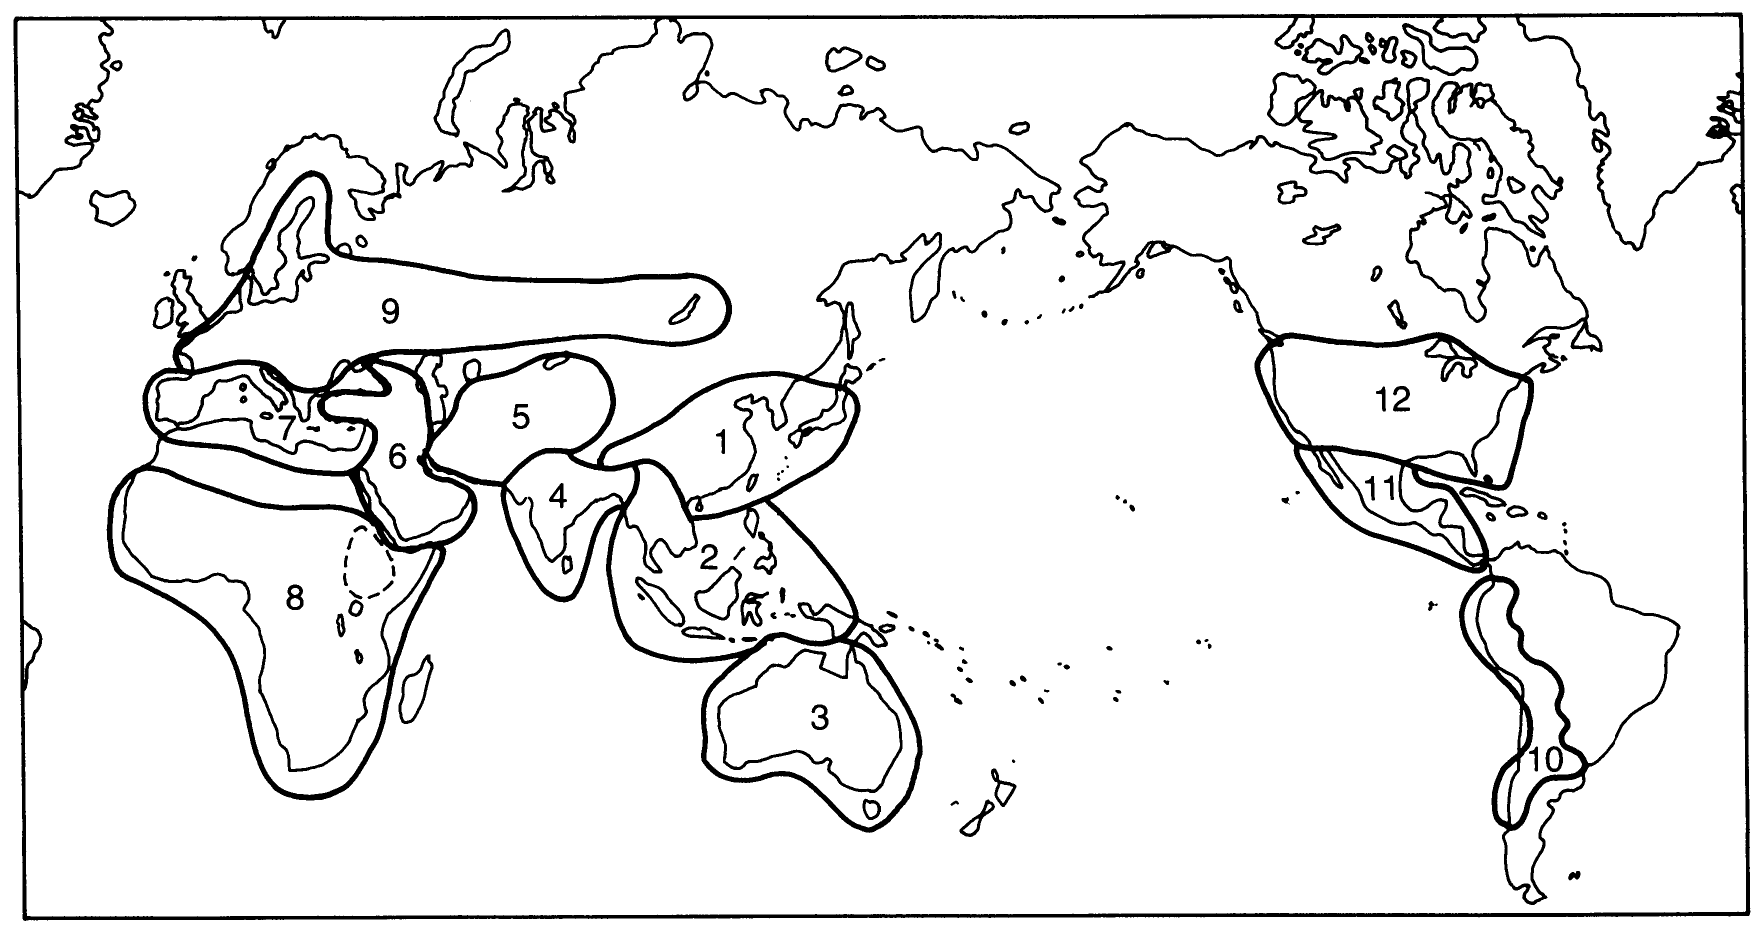
\includegraphics[width=0.7\textwidth, keepaspectratio,height=0.6\textheight]{./images/megacentres_cultivated} \caption{Megacentres of cultivated plants (Zeven and Zhukovsky, 1975); @hayward2012plant, Page 37}\label{fig:cultivated-megacentres-fig}
\end{figure}
\end{frame}

\begin{frame}{Megacentres of cultivated plants \ldots{}}
\protect\hypertarget{megacentres-of-cultivated-plants}{}
\begin{table}

\caption{\label{tab:cultivated-megacentres-tab}Cultivated plants and their regions of diversity. Based on Zeven and Zhukovsky (1975) and Zeven and de Wet (1982); @hayward2012plant, Page 54, 55.}
\centering
\fontsize{6}{8}\selectfont
\begin{tabular}[t]{>{\raggedright\arraybackslash}p{4em}>{\raggedright\arraybackslash}p{14em}>{\raggedright\arraybackslash}p{28em}}
\toprule
SN & Region & Crops\\
\midrule
\cellcolor{gray!6}{1} & \cellcolor{gray!6}{Chinese-Japanese region} & \cellcolor{gray!6}{Prosomillet, Foxtail millet, Naked oat}\\
 &  & Soybean, Adzuki bean\\
\cellcolor{gray!6}{} & \cellcolor{gray!6}{} & \cellcolor{gray!6}{Leafy mustard}\\
 &  & Orange/Citrus, Peach, Apricot, Litchi\\
\cellcolor{gray!6}{} & \cellcolor{gray!6}{} & \cellcolor{gray!6}{Bamboo, Ramie, Tung oil tree, Tea}\\
\addlinespace
2 & Indochinese-Indonesian region & Rice\\
\cellcolor{gray!6}{} & \cellcolor{gray!6}{} & \cellcolor{gray!6}{Rice bean, Winged bean}\\
 &  & Cucurbits/Ash gourd\\
\cellcolor{gray!6}{} & \cellcolor{gray!6}{} & \cellcolor{gray!6}{Mango, Banana, Rambutan, Durian, Bread fruit, Citrus/Lime, Grapefruit}\\
 &  & Bamboos, Nutmeg, Clove, Sago-palm, Ginger, Taros and Yams, Betel nut, Coconut\\
\addlinespace
\cellcolor{gray!6}{3} & \cellcolor{gray!6}{Australian region} & \cellcolor{gray!6}{Eucalyptus, Acacia, Macadamia nut}\\
4 & Hindustani region & Rice, Little millet\\
\cellcolor{gray!6}{} & \cellcolor{gray!6}{} & \cellcolor{gray!6}{Black gram, Green gram, Moth bean, Rice bean, Dolichos bean, Pigeonpea, Cowpea, Chickpea, Horsegram, Jute}\\
 &  & Eggplant, Okra, Cucumber, Leafy mustard, Rat's tail radish, Taros and Yams\\
\bottomrule
\end{tabular}
\end{table}
\end{frame}

\begin{frame}{}
\protect\hypertarget{section-7}{}
\begin{table}

\caption{\label{tab:cultivated-megacentres-tab2}Cultivated plants and their regions of diversity ...}
\centering
\fontsize{6}{8}\selectfont
\begin{tabular}[t]{>{\raggedright\arraybackslash}p{4em}>{\raggedright\arraybackslash}p{14em}>{\raggedright\arraybackslash}p{28em}}
\toprule
SN & Region & Crops\\
\midrule
\cellcolor{gray!6}{} & \cellcolor{gray!6}{} & \cellcolor{gray!6}{Citrus, Banana, Mango, Sunhemp, Tree cotton}\\
 &  & Sesame, Ginger, Turmeric, Cardamom, Arecanut, Sugarcane, Black pepper, Indigo\\
\cellcolor{gray!6}{5} & \cellcolor{gray!6}{Central Asian region} & \cellcolor{gray!6}{Wheat (Bread/Club/Shot), Rye}\\
 &  & Allium/Onion, Garlic, Spinach, Peas, Beetroot, Faba bean\\
\cellcolor{gray!6}{} & \cellcolor{gray!6}{} & \cellcolor{gray!6}{Lentil, Chickpea}\\
\addlinespace
 &  & Apricot, Plum, Pear, Apple, Walnut, Almond, Pistachio, Melon, Grape, Carrot, Radish\\
\cellcolor{gray!6}{} & \cellcolor{gray!6}{} & \cellcolor{gray!6}{Hemp/Cannabis, Sesame, Flax, Safflower}\\
6 & Near Eastern region & Wheat (Einkorn, Durum, Poulard, Bread), Barley, Rye/Secale\\
\cellcolor{gray!6}{} & \cellcolor{gray!6}{} & \cellcolor{gray!6}{Faba bean, Chickpea, French bean, Lentil, Pea}\\
 &  & Brassica oleracea, Allium, Melon, Grape, Plum, Pear, Apple, Apricot, Pistachio, Fig, Pomegranate, Almond\\
\addlinespace
\cellcolor{gray!6}{} & \cellcolor{gray!6}{} & \cellcolor{gray!6}{Safflower, Sesame, Flax}\\
 &  & Lupins, Medics\\
\cellcolor{gray!6}{7} & \cellcolor{gray!6}{Mediterranean region} & \cellcolor{gray!6}{Wheat (Durum, Turgidum), Oats}\\
 &  & Brassica oleracea, Lettuce, Beetroot, Colza\\
\cellcolor{gray!6}{} & \cellcolor{gray!6}{} & \cellcolor{gray!6}{Faba bean, Radish}\\
\addlinespace
 &  & Olive, Trifolium/Berseem, Lupins, Crocus, Grape, Fennel, Cumin, Celery, Linseed\\
\bottomrule
\end{tabular}
\end{table}
\end{frame}

\begin{frame}{}
\protect\hypertarget{section-8}{}
\begin{table}

\caption{\label{tab:cultivated-megacentres-tab3}Cultivated plants and their regions of diversity ...}
\centering
\fontsize{6}{8}\selectfont
\begin{tabular}[t]{>{\raggedright\arraybackslash}p{4em}>{\raggedright\arraybackslash}p{14em}>{\raggedright\arraybackslash}p{28em}}
\toprule
SN & Region & Crops\\
\midrule
\cellcolor{gray!6}{8} & \cellcolor{gray!6}{African region} & \cellcolor{gray!6}{Wheat (Durum, Emmer, Poulard, Bread)}\\
 &  & African rice, Sorghum, Pearl millet, Finger millet, Teff\\
\cellcolor{gray!6}{} & \cellcolor{gray!6}{} & \cellcolor{gray!6}{Cowpea, Bottle gourd, Okra, Yams, Cucumber}\\
 &  & Castor bean, Sesame, Niger, Oil palm, Safflower, Flax\\
\cellcolor{gray!6}{} & \cellcolor{gray!6}{} & \cellcolor{gray!6}{Cotton, Kenaf, Coffee}\\
\addlinespace
 &  & Kola, Bambara, Groundnut, Date palm, Ensete, Melons\\
\cellcolor{gray!6}{9} & \cellcolor{gray!6}{European-siberian region} & \cellcolor{gray!6}{Peach, Pear, Plum, Apricot, Apple, Almond, Walnut, Pistachio, Cherry}\\
 &  & Cannabis, Mustard (black), Chicory, Hops, Lettuce\\
\cellcolor{gray!6}{10} & \cellcolor{gray!6}{South American region} & \cellcolor{gray!6}{Potato, Sweet potato, Xanthosoma}\\
 &  & Lima bean, Amaranth, Chenopodium, Cucurbita, Tomato, Tobacco, Lupin\\
\addlinespace
\cellcolor{gray!6}{} & \cellcolor{gray!6}{} & \cellcolor{gray!6}{Papaya, Pineapple}\\
 &  & Groundnut, Sea island cotton\\
\cellcolor{gray!6}{} & \cellcolor{gray!6}{} & \cellcolor{gray!6}{Cassava, Cacao, Rubber tree, Passion fruit}\\
11 & Central American and Mexican region & Maize, French bean, Potato, Cucurbita, Pepper/Chilli, Amaranth, Chenopodium, Tobacco, Sisal hemp, Upland cotton\\
\cellcolor{gray!6}{12} & \cellcolor{gray!6}{North American region} & \cellcolor{gray!6}{Jeruselum artichoke, Sunflower, Plum, Raspberry, Strawberry}\\
\bottomrule
\end{tabular}
\end{table}
\end{frame}

\begin{frame}{Plant introduction}
\protect\hypertarget{plant-introduction}{}
\begin{itemize}
\item
  The plant breeder may import new, unadapted genotypes from outside the
  production region, usually from another country (called plant
  introductions). These new materials may be evaluated and adapted to
  new production regions as new cultivars, or used as parents for
  crossing in breeding projects.
\item
  Primary Introduction

  \begin{itemize}
  \tightlist
  \item
    When the introduced variety is well adapted to the new environment,
    it is released for commercial cultivating without any alteration in
    the original genotype; this constitutes primary introduction. It is
    less common, particularly in countries having well organized crop
    improvement programmes.
  \end{itemize}
\item
  Secondary introduction

  \begin{itemize}
  \tightlist
  \item
    The introduced variety may be subject to selection in order to
    isolate a superior variety. Alternatively, it may be hybridized with
    local varieties to transfer one or few characters from these
    varieties to the local ones. Such introduction constitutes secondary
    introduction. It is much common than primary introduction.
  \end{itemize}
\end{itemize}
\end{frame}

\begin{frame}{Purpose of plant introduction}
\protect\hypertarget{purpose-of-plant-introduction}{}
\begin{enumerate}
\tightlist
\item
  To obtain entirely new crop species
\item
  To serve as new varieties
\item
  For use in crop improvement programmes
\item
  To introgress variability to existing genetic materials
\item
  For scientific studies
\item
  To augment aesthetics
\item
  For germplasm collection and comparison
\end{enumerate}
\end{frame}

\begin{frame}{Acclimatization}
\protect\hypertarget{acclimatization}{}
\begin{itemize}
\item
  Acclimatization is the reversible process by which an individual
  becomes adapted to a change in the environment, often involving
  temperature, moisture, food, often relating to seasonal climate
  changes. The process that leads to the adaptation of a variety, line
  or population to a new environment is known as acclimatization.
  Acclimatization is characterized by a faster multiplication of those
  genotypes -- adaptive fitness -- (present in the original population)
  that are better adapted to the new environment.
\item
  Factors affecting extent of acclimatization:

  \begin{enumerate}
  \tightlist
  \item
    Mode of pollination
  \item
    The magnitude of genetic variability present in the original
    population
  \item
    The duration of life cycle of the crop
  \item
    Tendency to acquire and augment mutation
  \item
    Nature and intensity of environmental stresses
  \end{enumerate}
\end{itemize}
\end{frame}

\hypertarget{other-steps-in-plant-breeding}{%
\section{Other steps in plant
breeding}\label{other-steps-in-plant-breeding}}

\begin{frame}{Germplasm collection}
\protect\hypertarget{germplasm-collection}{}
\footnotesize

\begin{itemize}
\tightlist
\item
  These resources may take the form of seed collections stored in seed
  banks, trees growing in nurseries, animal breeding lines maintained in
  animal breeding programs or gene banks, etc.
\item
  Three principles guide the collection, conservation and
  exchange/utilization of germplasm:

  \begin{itemize}
  \tightlist
  \item
    \footnotesize When an accession is gathered a sample is left in the
    country of origin for national use
  \item
    Germplasm is made freely available to all bona fide workers
  \item
    All long term collections are duplicated and maintained in another
    location.
  \end{itemize}
\item
  Range from collections of wild species to elite, domesticated breeding
  lines that have undergone extensive human selection.
\item
  Important for

  \begin{itemize}
  \tightlist
  \item
    \footnotesize Maintenance of biological diversity and food security
  \item
    At times of crisis; irish famine (potato line was result of only a
    handful of introductions) and \emph{Helminthosporium} leaf blight in
    corn in US 1970s (Parental line of the popular hybrid maize was
    susceptible to disease.)
  \end{itemize}
\item
  Loss of genetic diversity has accelerated in recent decades, with many
  crops growing susceptible to diseases, pests and environmental
  stresses.
\item
  Germplasm collections are backed up by their characterizations --
  using technical guidelines and crop specific descriptors
  \footnote[frame]{\url{https://www.genebanks.org/resources/publications/key-access-and-utilization-descriptors-for-rice-genetic-resources/}}.
\end{itemize}
\end{frame}

\begin{frame}{Germplasm conservation}
\protect\hypertarget{germplasm-conservation}{}
\begin{columns}[T, onlytextwidth]

\column{0.5\textwidth}
\footnotesize
\begin{itemize}
\item Before being placed in cold storage, the sample is often multiplied so as to retain sufficient seeds or vegetative materials for storage and to send to other institutions.
\item Germplasm of crops grown from true seed is stored in 3 main types of banks:
  \begin{itemize}
  \footnotesize
  \item Long term gene banks, aka. base collections, stored at -10 to -20 degree C for several decades or upto century.
  \item Medium term banks, 0 - 5 degree C for upto 20 years.
  \item Short term collections, under 5 degree C for a few years.
  \end{itemize}
\end{itemize}

\column{0.5\textwidth}

\begin{figure}
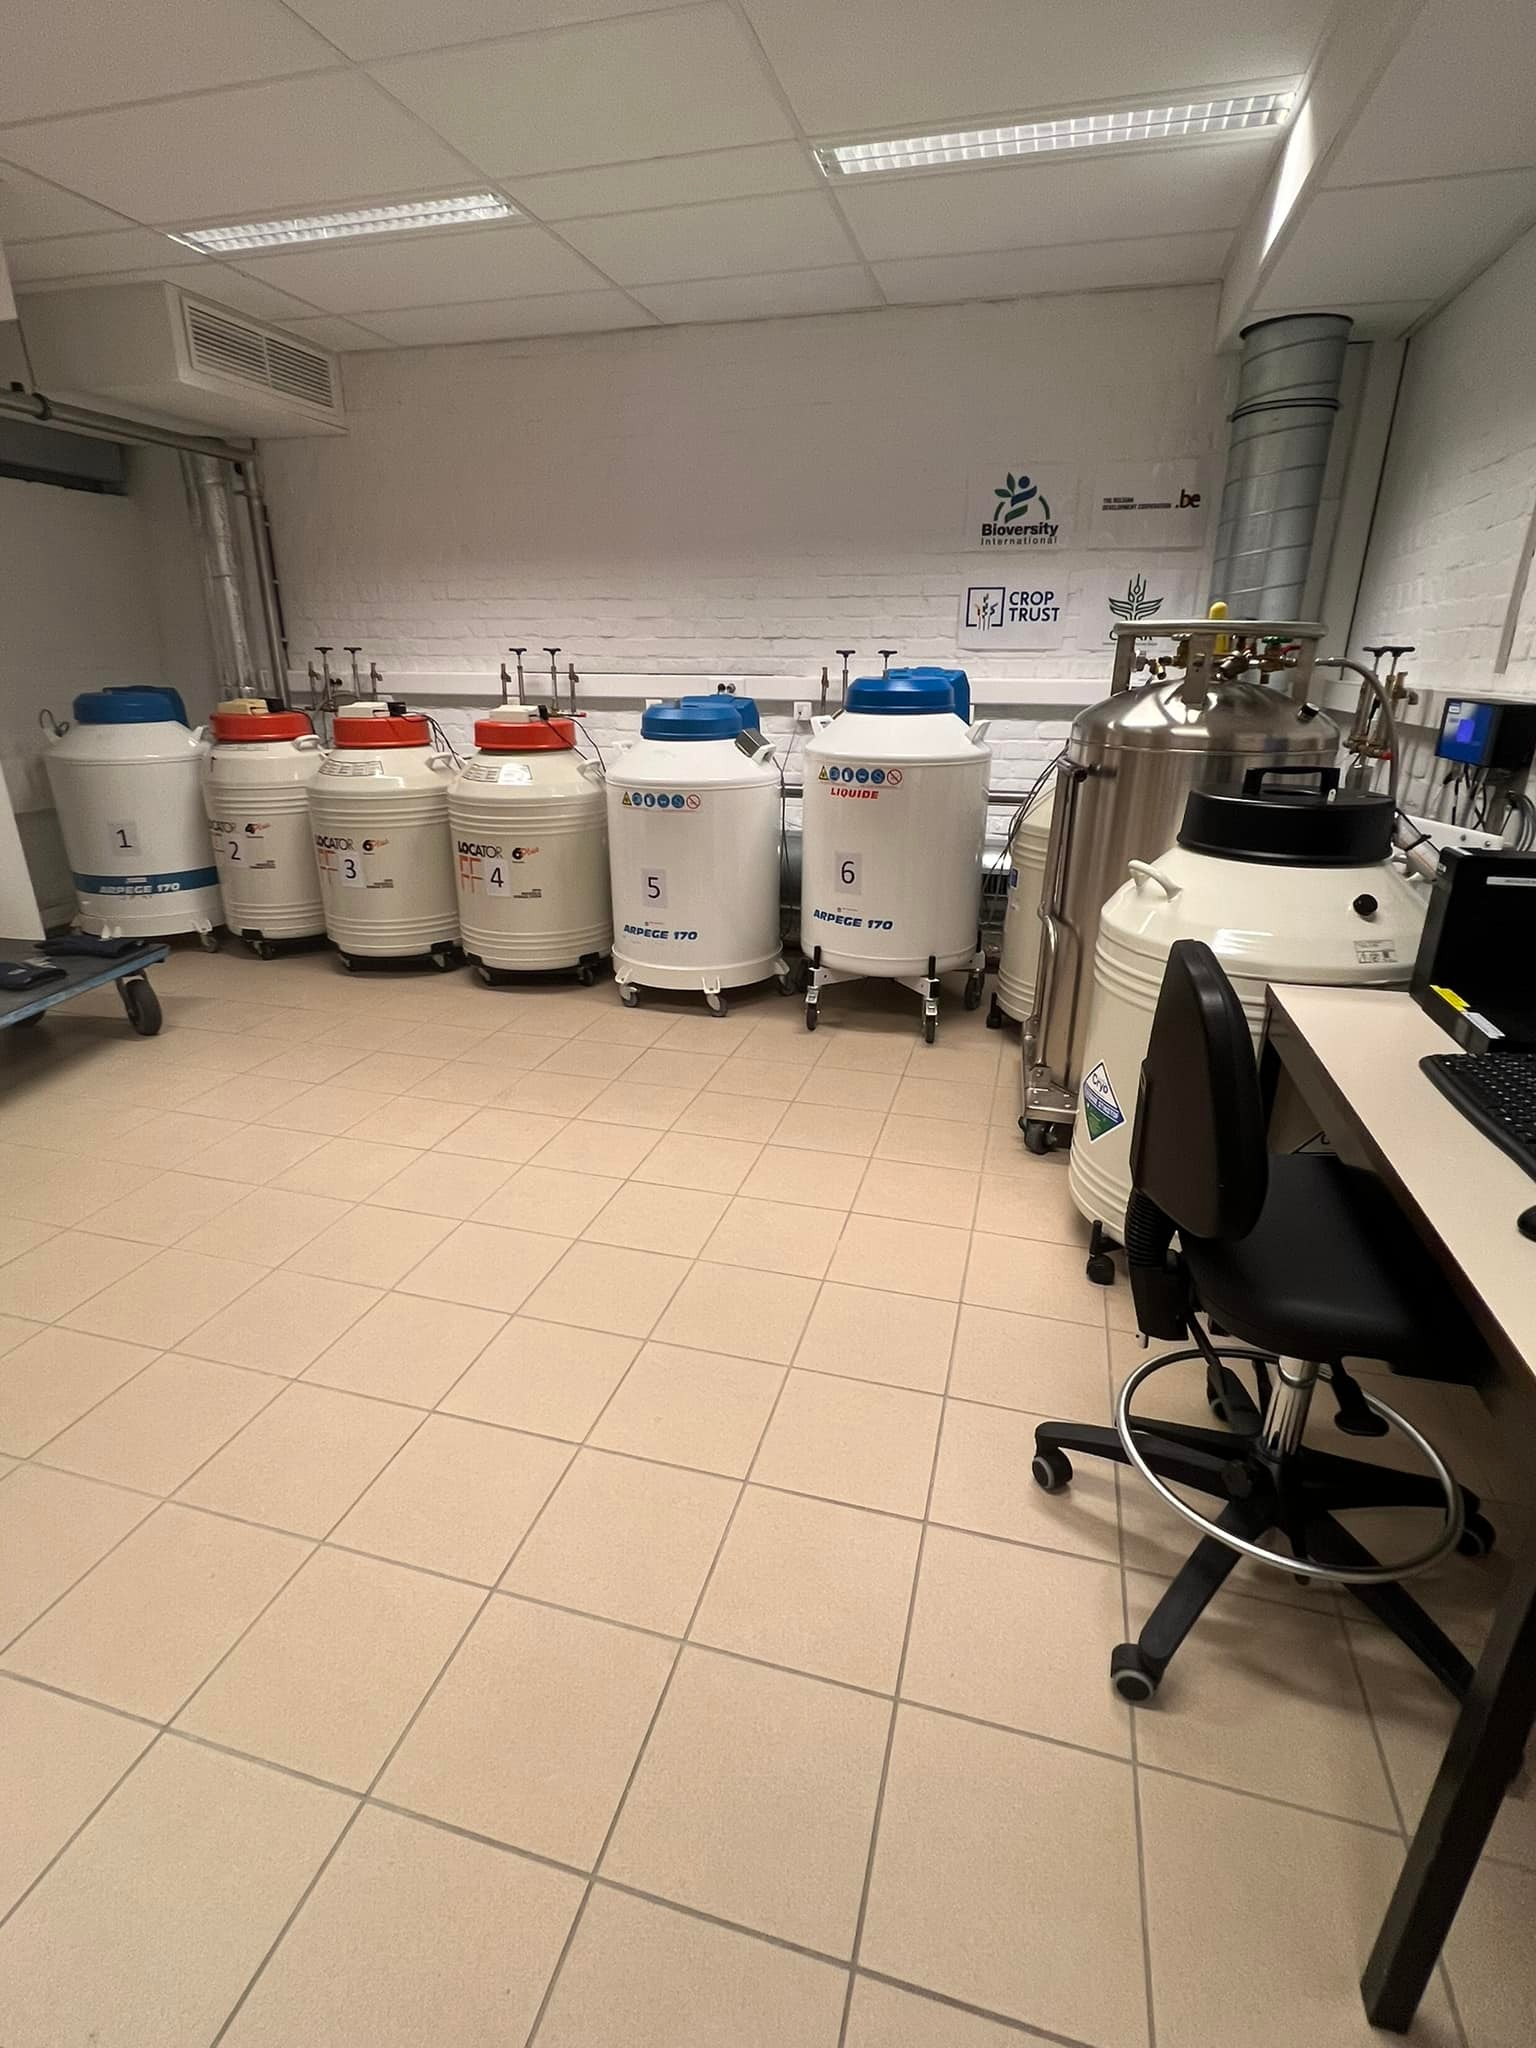
\includegraphics[width=0.6\linewidth]{./images/cryo-tanks-banana} \caption{Cryotanks for conservation of global banana germplasm.}\label{fig:cryo-tank-banana}
\end{figure}

\end{columns}
\end{frame}

\begin{frame}{Conservation: a case of rice}
\protect\hypertarget{conservation-a-case-of-rice}{}
\footnotesize

\begin{itemize}
\tightlist
\item
  Traditional rice varieties and wild rice species are being lost
  through genetic erosion and habitat loss. Farmers often adopt new,
  modern rice varieties, which displace older varieties.
\item
  Wild rice species are particularly threatened with extinction as their
  natural habitats are under threat or destroyed.
\item
  The most common, efficient and cheap method of conservation of rice
  diversity is in seed banks at low temperature (\(2^\circ C\) to
  \(-20^\circ C\)) and dry (moisture content of 6--7\% fresh weight).
  Most cultivated rice accessions are conserved in seed banks.
\item
  Field genebanks are needed for wild rice and related genera:

  \begin{itemize}
  \tightlist
  \item
    \footnotesize that produce recalcitrant seeds or no seeds. This is
    the case of \emph{O. longistaminata}, \emph{O. neocaledonica},
    \emph{O. granulata}, \emph{O. meyeriana} and related genera such as
    \emph{Leersia}, which do not produce enough seeds for storage.
    \emph{Porteresia coarctata} has recalcitrant seeds.
  \item
    that do not flower in genebank regeneration conditions. This is the
    case of O. schlechteri and related genera such as Potamophila and
    Zizaniopsis at IRRI.
  \item
    that have special needs, where different species require different
    cultural practices. \emph{O. granulata} and \emph{O. meyeriana} for
    example, need partial shading and special soils, because they are
    originally from forest regions, whereas most of the other species
    need to be kept soaked because they are originally from swampy
    areas.
  \end{itemize}
\end{itemize}
\end{frame}

\begin{frame}{}
\protect\hypertarget{section-9}{}
\begin{itemize}
\tightlist
\item
  More than 780,000 accessions of cultivated and wild rice are stored in
  genebanks in more than 40 countries. However, many of these accessions
  are duplicates, so this number does not represent numbers of distinct
  varieties.
\item
  Major rice collections in CGIAR are maintained by the International
  Rice Research Institute (IRRI) and AfricaRice. CIAT maintains a
  working collection used for breeding rice for Latin American
  countries.
\item
  Other large collections are conserved at CAAS in China, which holds
  the largest collection of wild rice and related genera, Russia and the
  USA.
\end{itemize}
\end{frame}

\begin{frame}{Germplasm utilization}
\protect\hypertarget{germplasm-utilization}{}
\end{frame}

\hypertarget{the-vavilov-concept}{%
\section{The Vavilov Concept}\label{the-vavilov-concept}}

\begin{frame}{}
\protect\hypertarget{section-10}{}
\begin{itemize}
\item
  Nikolai I. Vavilov (1887-1942), the Russian botanist and plant
  breeder, demonstrated the existence of `centres of origin' of
  cultivated plants (more correctly named today as `centres of
  diversity'), in which can be found the highest level of genetic
  variability of a species. This variability, which arises in nature by
  mutation spontaneous hybridization, introgression and changes in
  chromosome form and number, provides the means by which adaptation to
  heterogenous environments can occur.
\item
  It allows the breeder to identify sources of variation for specific
  characteristics. The extension of this principle to related species
  was formulated by Vavilov in his `law of homologous series of
  variation.' This law allows the prediction of the appearance of a
  given type of mutation in a plant species when such a type has been
  found in another species phylogenetically related to the first. As a
  result of his studies Vavilov defined plant breeding as `plant
  evolution directed by man.' He recognized that in a breeding
  programme, by growing variable populations in conditions favouring the
  expression of the characters, selection may be facilitated. Also, by
  creating variability in a parallel way to nature the breeder exploits
  genetical methods. Plant breeding can thus also be defined as `applied
  plant genetics.'
\end{itemize}
\end{frame}




\end{document}
